%%% Local Variables:
%%% mode: latex
%%% TeX-master: "../doc"
%%% coding: utf-8
%%% End:
% !TEX TS-program = pdflatexmk
% !TEX encoding = UTF-8 Unicode
% !TEX root = ../doc.tex

This sections explains the fundamental technologies and achievements from previous projects which have been applied in the project.

\section{Technological prototype} \label{Prototype}
As mentioned in chapter \ref{Initial position}, a technological prototype for the ATP has already been developed in a bachelor thesis during the previous semester. The prototype has been realized as a locally running application using the ASP.NET Core Blazor framework \cite{bachelorarbeit_Egger_Verstappen_page4}. The application fetches time data from Toggl Track via the Toggl Track API and relies on Local Storage for storing the application state. The graphical user interface has been designed with elements from the Bootstrap toolkit. Charts.js is used to display graphs and charts. The application is made available as a Docker image which can be downloaded from the GitHub Container Registry. As to software testing, unit tests for the part managing the communication between the application and Toggl have been implemented and can be run automatically via GitHub Actions. \cite{bachelorarbeit_Egger_Verstappen_page23-25}.

The different features, however, have not been fully implemented yet. The charts display dummy data instead of real time data, as shown in figure \ref{figure1}. The tracked time data can be retrieved from Toggl, but no further action is applied to it. Local Storage is not considered to be suitable for application data storage on the long term. Further possible enhancements include localization, accessing other APIs and not just Toggl, different installation and update strategies as well as additional automated tests like UI tests and integration tests. \cite{bachelorarbeit_Egger_Verstappen_page26-27}

\begin{figure}[H]
\centering
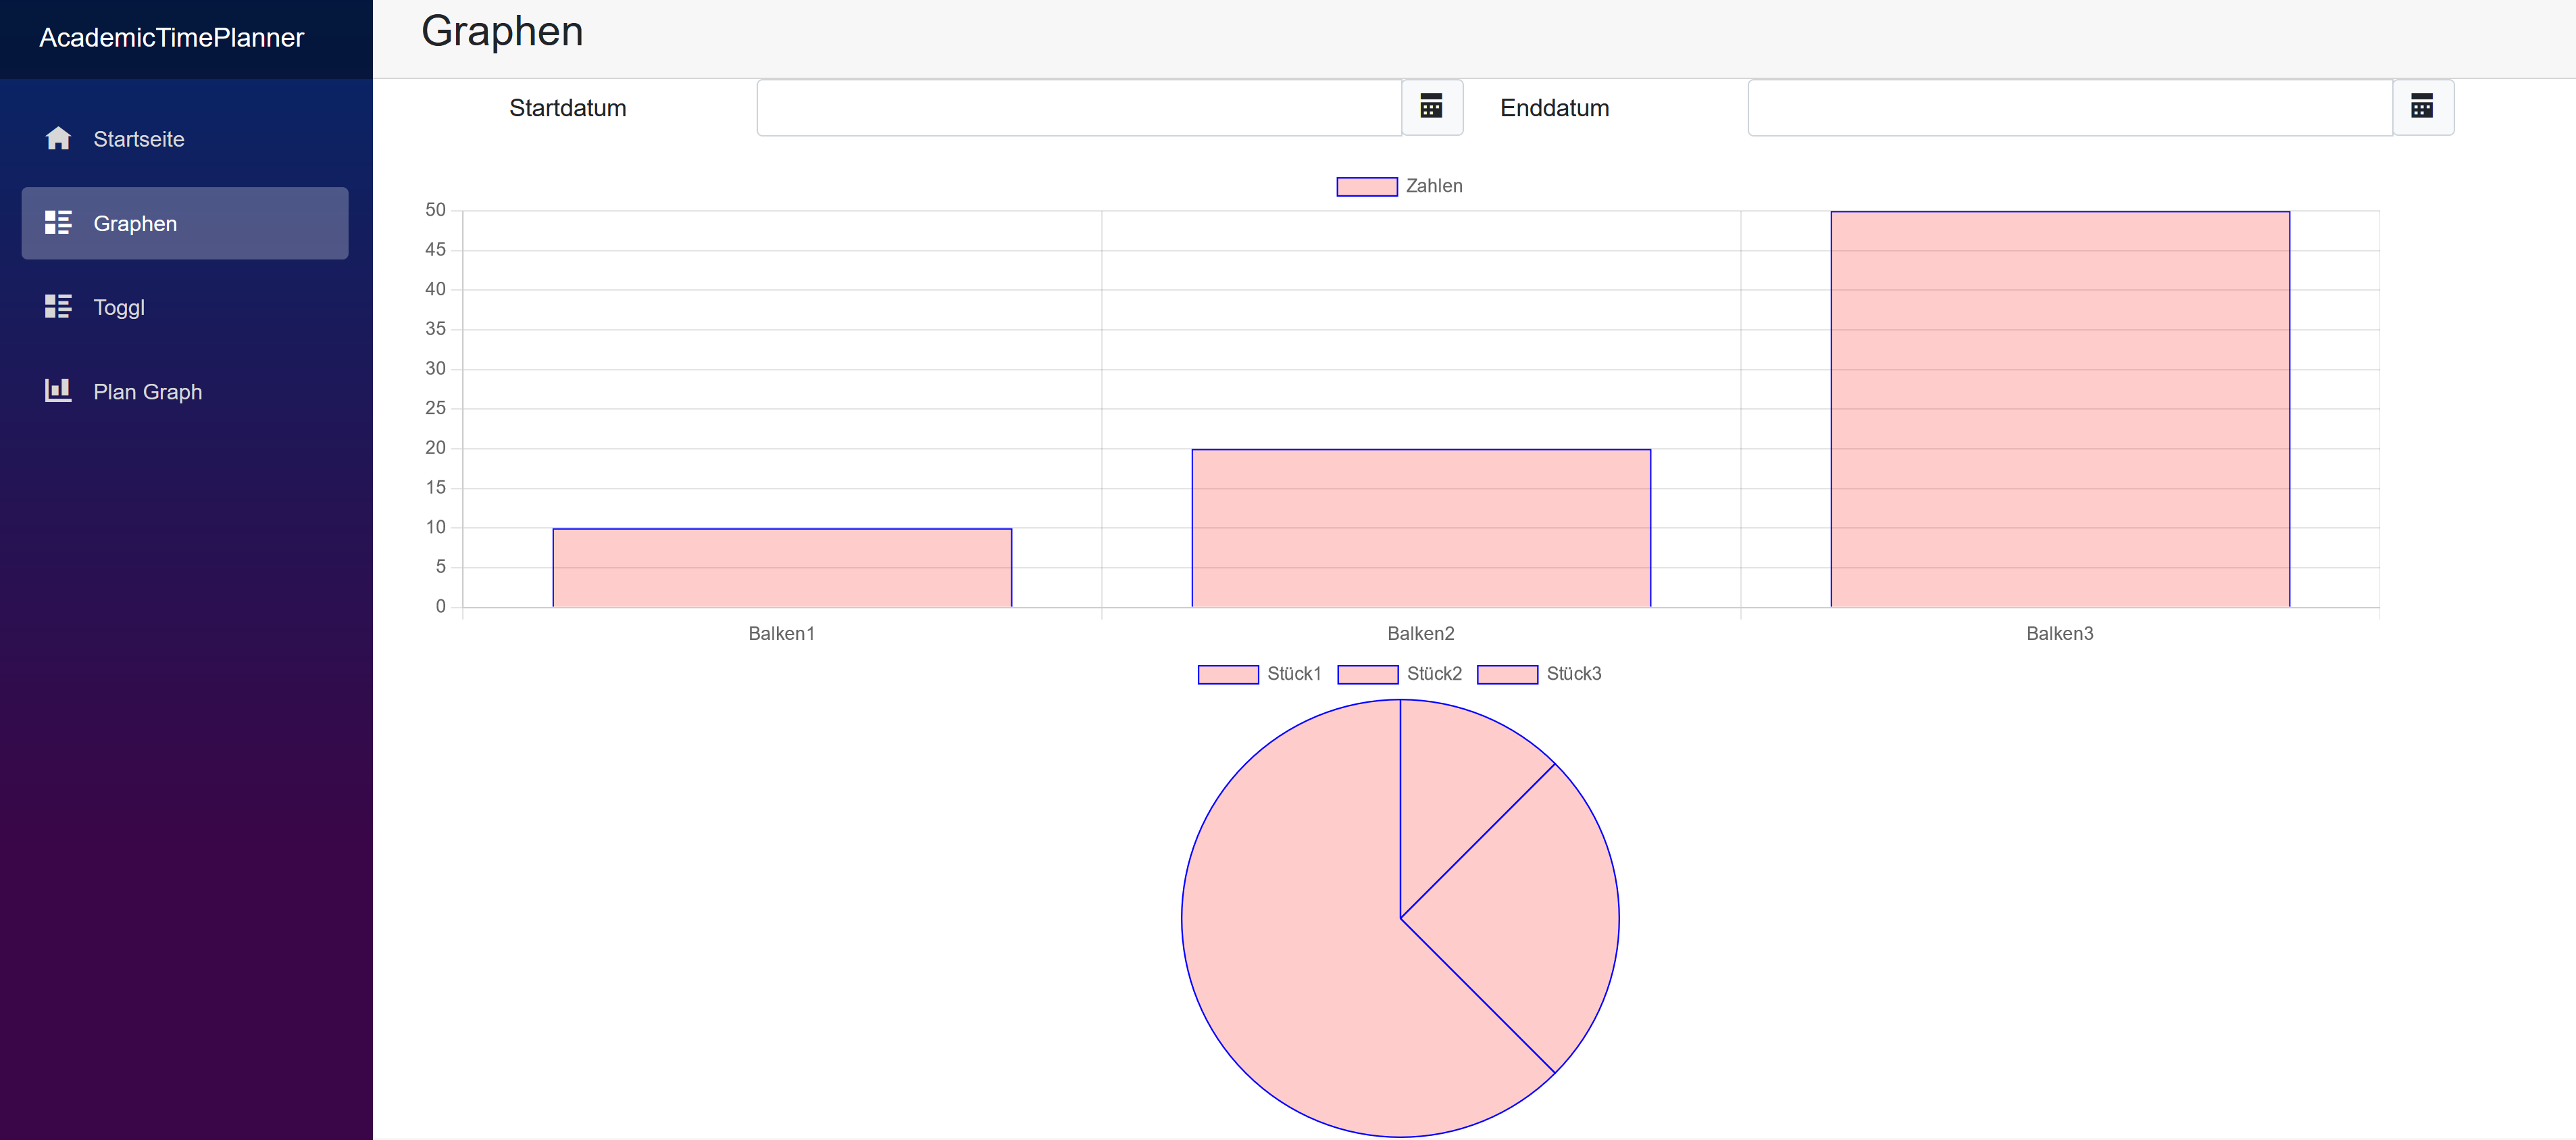
\includegraphics[width=1.0\columnwidth]{figure1_prototype_charts}
\caption{ATP prototype displaying dummy charts}
\label{figure1}
\end{figure}

\section{Toggl Track}
Toggl Track is an easy-to-use, multifunctional online time tracking application. Tasks can be tracked and grouped into projects. Tracking can be started and stopped using start and stop buttons. Times can also be manually entered and assigned to a task and a project. Toggl Track offers many additional functionalities including billing and invoicing, payroll calculating, generation of detailed reports and project budgeting. Toggl Track can be used on different devices like computers, smartphones and tablets. The tracking data is then synchronized between the devices. Furthermore, Toggl Track provides an API to be used to query tracked time entries from Toggl Track which can then be used outside Toggl Track itself, e. g. by other applications. \cite{bachelorarbeit_Egger_Verstappen_page8} \cite{toggl_track_url}

\section{Mapping Concept} \label{Mapping concept}
The mapping concept developed in the aforementioned bachelor thesis \cite{bachelorarbeit_Egger_Verstappen_page20-22} laid the foundation for this project. It determined how the data structure would be built and how the application would interact with Toggl Track. The concept was split into three entities; Plan, Toggl, and Budget and Group. 

\begin{figure}[H]
	\centering
	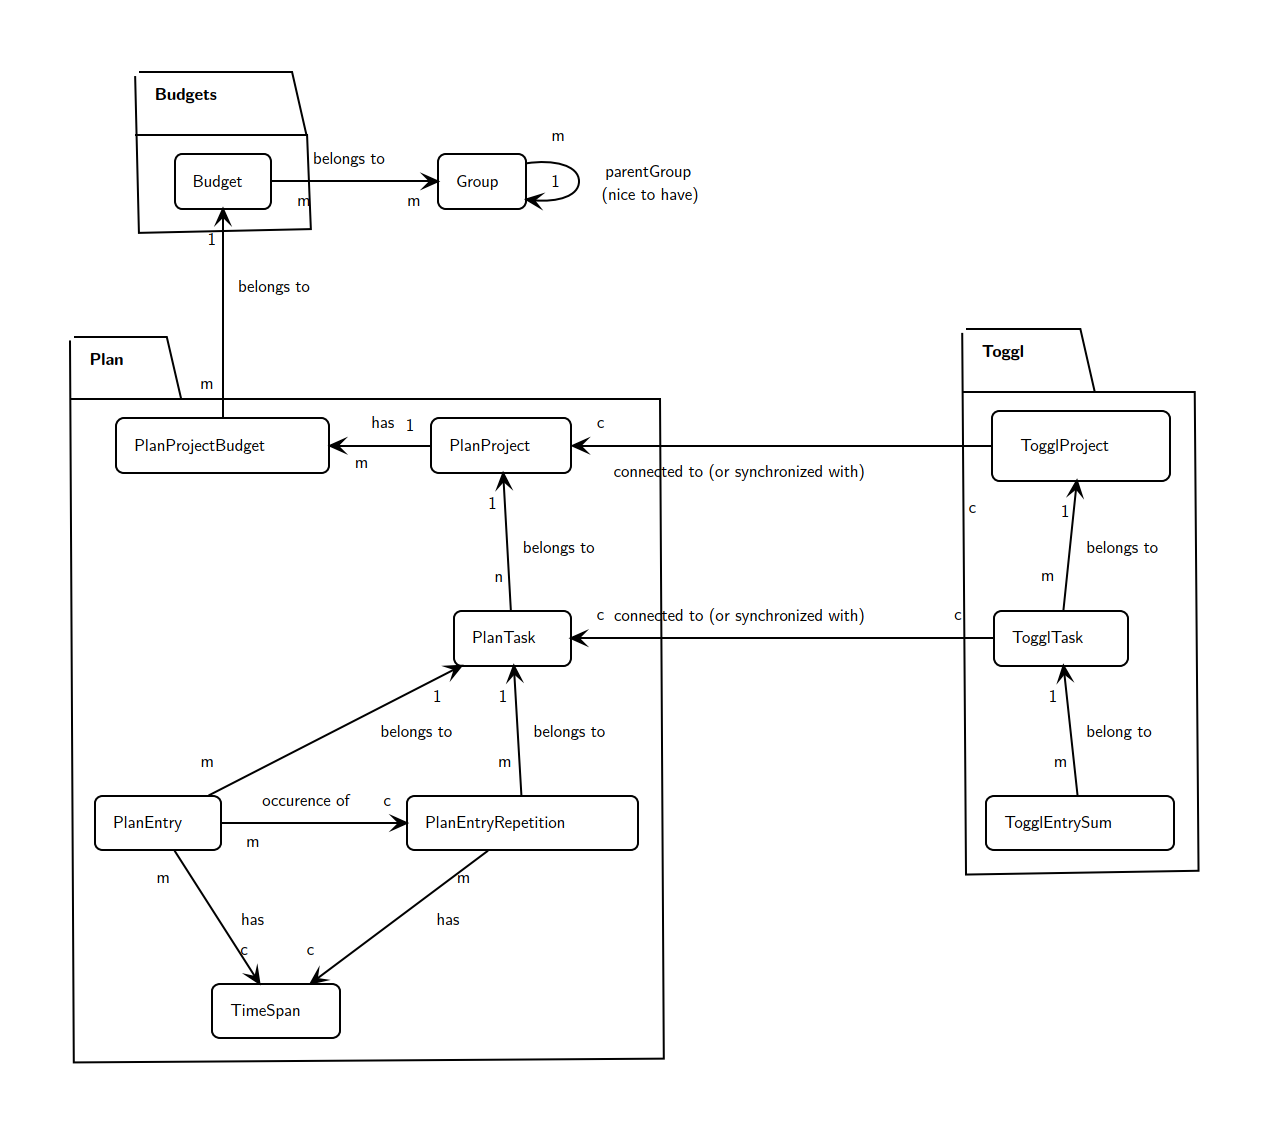
\includegraphics[width=1.0\columnwidth]{entitydiagram_prototype}
	\caption{Entity Relationship Diagram of the bachelor thesis prototype}
	\label{figure2}
\end{figure}

\subsection{Plan}
The plan consists of a plan entry which has a start and an end date as well as a time span. Start and end date denote in which time frame the task is planned, whereby the smallest unit of time is a day. The time span represents the time investment predicted for the task and has a unit of hours. This time span does not have to match the duration between start and end date and can be shorter.
\subsection{Toggl}
To save the data provided by Toggl, three entities are proposed in the bachelor thesis. Those entities save only the data needed by the ATP. They have an attribute togglId which corresponds with the ID given by Toggl. To compare the data of the plan project or the plan task with the tracked time, TogglProject and TogglTask were defined. The time captured in Toggl can be saved in the TogglEntrySum.

\begin{figure}[H]
	\centering
	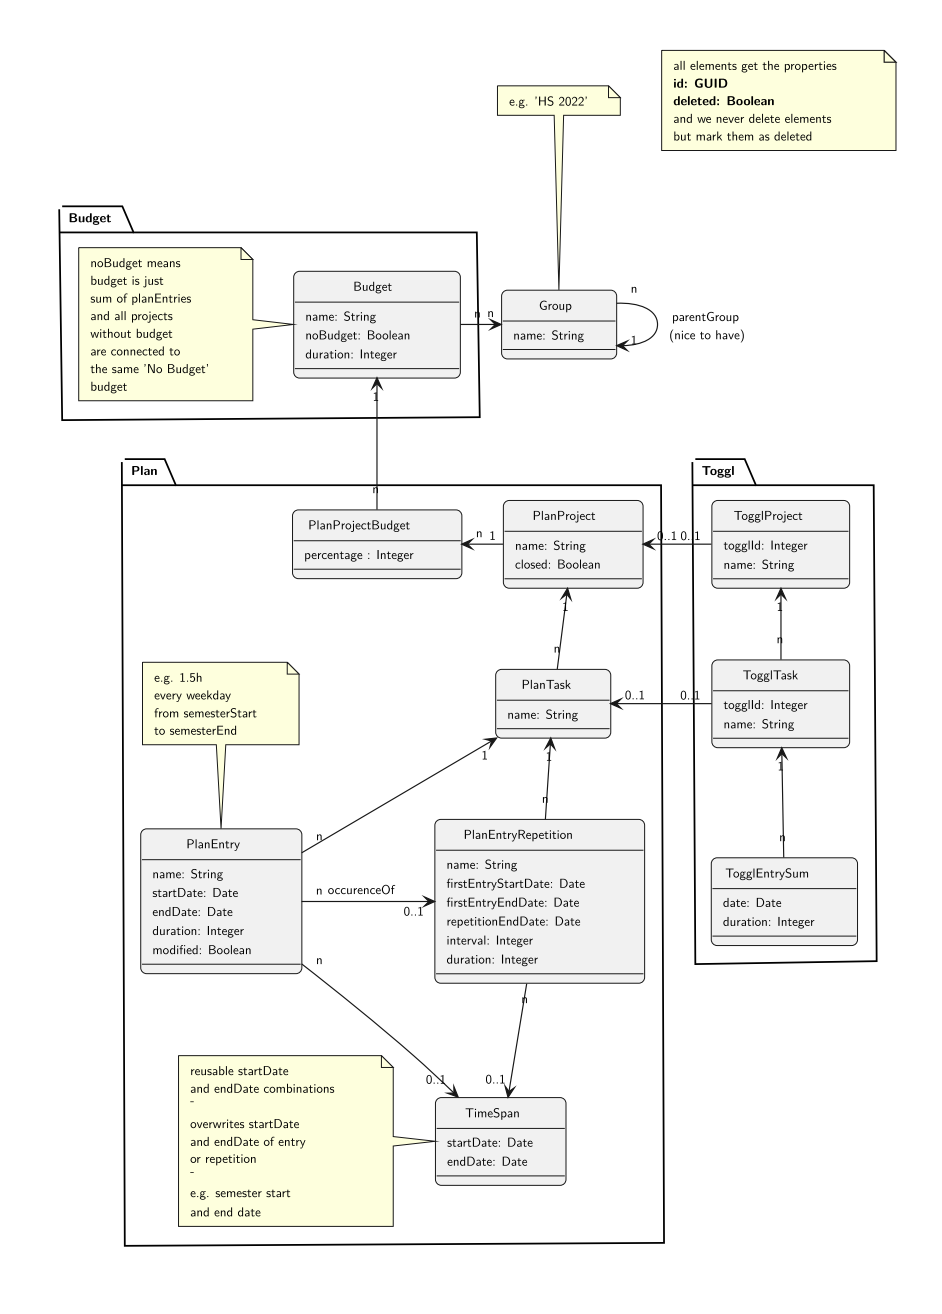
\includegraphics[width=1.0\columnwidth]{classdiagram_prototype}
	\caption{Class Diagram of the bachelor thesis prototype}
	\label{figure3}
\end{figure}

\subsection{Budget and Group}
Budgets are optional features of the ATP. They are used if a task does not have an equal distribution. For instance, the budgets allow a lecturer to allocate more time for preparing and marking of exam papers. The budgets can be divided into groups like semester or year.

\section{GitHub} \label{GitHub}
GitHub \cite{github_url} is an online service which provides Git \cite{git_url} based version control for software projects.
\subsection{Version control} \label{Version control}
Version control is used to see what was changed when and by whom. It can also be used to roll back to an older state if needed. In GitHub a feature branch is created to implement a certain feature, and afterwards when finished such a branch will be integrated into the main branch via a pull request. This pull request allows the other members of the team to request changes before the branch is merged into the main branch. This process also enables members of a team to work independently without the problem of accidentally interfering with an other team member's work.
\subsection{GitHub Actions} \label{GitHub Actions}
GitHub Actions is a (CI/CD) platform \cite{github_actions_url}. It allows for build and test automation as well as maintaining a deployment pipeline. Furthermore, workflows to automatically test and build the software on every pull request can be created. This feature helps to prevent the accidental inclusion of broken features or features which isolated work as intended but would cause other parts of the software to crash when integrated into it.
\subsection{GitHub Issues} \label{GitHub Issues}
Issues are often related to features and the corresponding feature branches. They provide the possibility to break down a milestone into manageable tasks which can then be assigned to the members of the team to work on. Thus, tasks and their assigned members can be monitored and identified. 

\section{JSON}
JSON (JavaScript Object Notation) \cite{json_url} is a data-interchange format. JSON is easily readable by humans and machines alike. It is also easy to write/generate a JSON file. Furthermore, it is language independent.\newline
JSON consists of two structures:
\begin{itemize}
	\item A collection of unordered name/value pairs. They are enclosed in curly brackets. A pair is seperated by a colon and after each name/value pair, a comma follows to separate them from the next pair.
	\item An ordered list of variables. Such a list starts with a left and ends with a right square bracket.
\end{itemize}
These two structures can be combined in a JSON file to get something akin to the JSON file shown in picture \ref{figure4}

\begin{figure}[H]
	\centering
	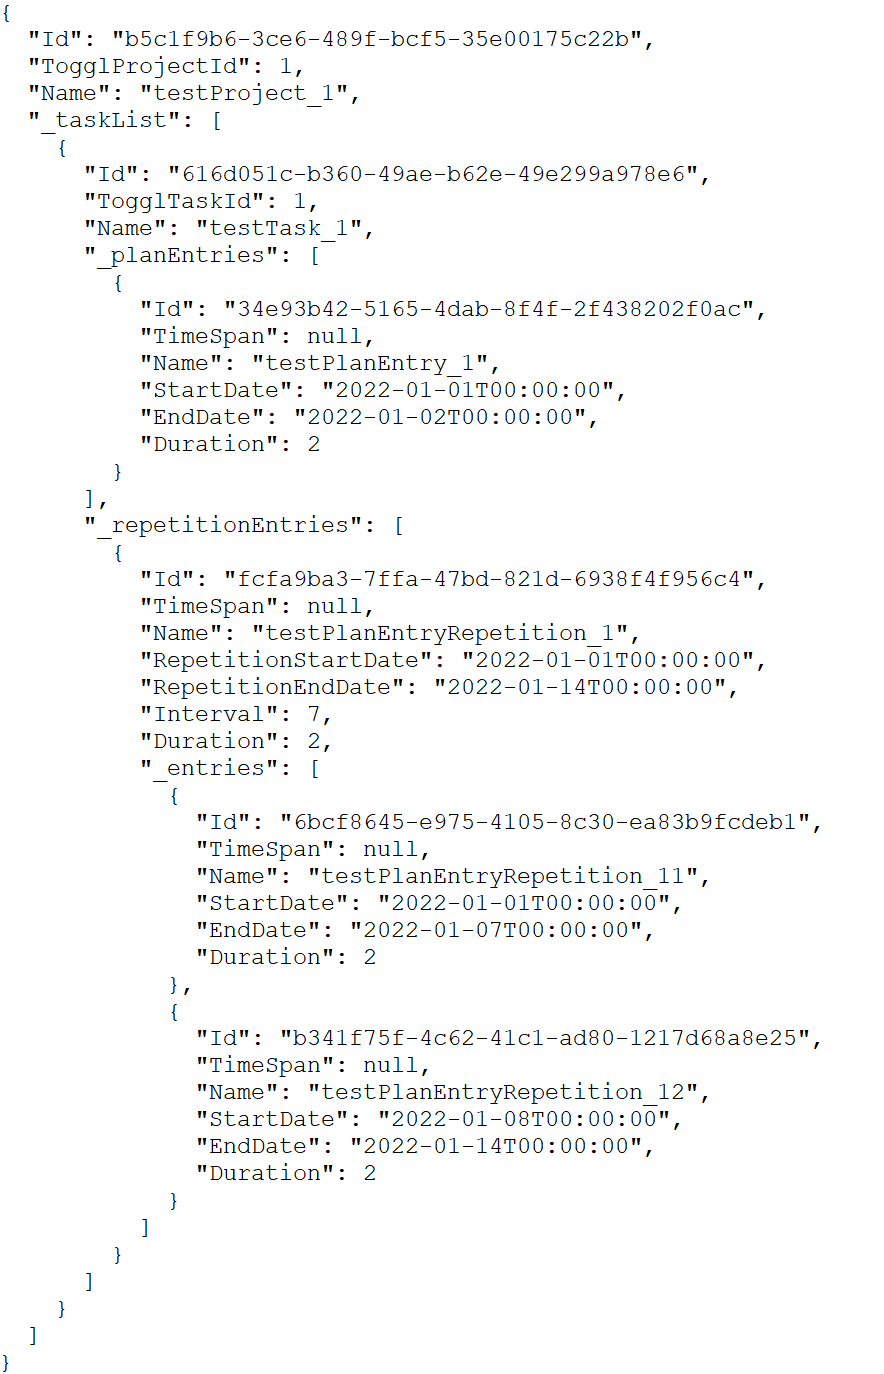
\includegraphics[width=0.7\columnwidth]{JSONExample}
	\caption{Example of a JSON file}
	\label{figure4}
\end{figure}

\section{Local Storage} \label{Local Storage}
Local Storage is a mechanism provided by the Web Storage API by which browsers can store data as key/value pairs without having to use cookies. Data stored in Local Storage persists when the browser is closed and reopened and only is deleted on cache clearing \cite{web-storage-api-url}. Moreover, the data is scoped to the browser window, which means that multiple tabs within the same browser window share the data \cite{blazor-state-management-url}. The maximum amount of data which can be stored in Local Storage is 5 MB. To access Local Storage from within a Blazor application, there is an open-source library available, which is called LocalStorage and provided by Blazored \cite{local-storage-url}.

\section{C\#}
C\# is "[...] a powerful and widely used programming language that you can use to make websites, games, mobile apps, desktop apps and more with .NET. [...]" \cite{csharp-url}.